\documentclass[11pt]{article}
\usepackage[margin=1in]{geometry}
\usepackage{amsmath,amssymb,amsthm}
\usepackage{booktabs}
\usepackage{graphicx}
\usepackage[hidelinks]{hyperref}
\newtheorem{theorem}{Theorem}

\title{\textbf{Designing Novel, Safe, and Pleasant Flavors:\\ A Structure--Receptor--Percept
Pipeline with a Machine-Checked Tastiness Metric}}
\author{Anonymous Author(s)\\ \small Submission under double-blind review}
\date{}

\begin{document}
\maketitle

\begin{abstract}
Motivated by the conjecture that exceptional, never-experienced flavors exist in a vast
molecular flavor space, we build a computational pipeline for designing novel flavor
combinations. The pipeline follows the biological chain \emph{molecule $\rightarrow$
odorant-receptor activation $\rightarrow$ perceived flavor}: (i) a structure-based model
predicts human panel \emph{pleasantness} (5-fold CV Spearman $0.50$ on 420 molecules from
Keller \& Vosshall 2016); (ii) an odorant-receptor layer grounded in the Mainland 2015 screen
provides a real, if partial, receptor signal ($1.57\times$ chance that structurally nearest
molecules share a receptor); (iii) a food-appropriate toxicity screen filters hazardous
structures (drug-discovery filters such as Brenk/PAINS are shown to be miscalibrated for
food); (iv) a fragment-based (BRICS) generator constructs \emph{de novo} molecules, of which
the top candidates are all absent from PubChem; and (v) a compositional-statistics model
learns which chemical classes drive pleasantness (lactones/esters up, sulfur/acids down;
composition predicts blend pleasantness at Spearman $0.42$) and steers a multi-objective
generator that maximizes predicted pleasantness and novelty while minimizing toxicity. We
show a learned non-additive mixture model captures interaction that mean-pooling cannot
($0.82$ vs $0.25$ Spearman on a controlled non-additive oracle), and we \emph{machine-check
in Lean} the key property that under an additive score no blend can exceed its best
component. This formalizes precisely why non-additive modeling is required. We are explicit about
scope: outputs are computational hypotheses for a chemist or molecular gastronomist, not
safety-cleared recipes, and human validation remains future work.
\end{abstract}

\section{Introduction}
Most single flavors are one molecule (vanillin, isoamyl acetate), but chocolate is a
high-dimensional mixture of hundreds of odor-active compounds acting across roughly $30$ taste
and $400$ odor receptors. If flavor space is that large and mostly unexplored, exceptional
flavors that no human has tasted plausibly exist. This work operationalizes that idea as a
design problem: learn what tastes good, generate new molecules, and blend them into novel,
safe, pleasant recipes, with every claim tied to public data or a stated control. The
conjecture and framing are due to a recent essay on biological challenges for AI; our
contribution is the computational instrument and its honest evaluation.

\section{Related work}
Structure-to-odor prediction has advanced from chemoinformatic baselines (the DREAM Olfaction
Challenge) to learned embeddings that reach human-level odor labeling (the Principal Odor Map).
Odorant receptors are G-protein-coupled receptors; receptor screens (Mainland 2015) and
resources such as GPCRdb connect the flavor and pharmacology sides. Pleasantness (hedonic
valence) is a primary perceptual dimension of olfaction. We build on these with real labeled
data (via Pyrfume) and add de-novo generation, a food-appropriate safety screen, a learned
mixture model, compositional statistics, and a machine-checked metric.

\section{Methods}
\textbf{Data.} Real molecules and pleasantness labels from Keller \& Vosshall 2016; odor
descriptors from Leffingwell; odorant-receptor activations from Mainland 2015; all via Pyrfume.
Molecules are featurized as ECFP4 fingerprints.

\textbf{Goodness model.} A random forest maps ECFP4 to panel pleasantness, evaluated by 5-fold
cross-validated Spearman/$R^2$.

\textbf{Receptor layer.} Confirmed molecule--OR activations provide known receptor hits; a
structural nearest-neighbour predictor infers likely activation, validated leave-one-out
against a chance baseline.

\textbf{Toxicity screen.} A curated denylist, genotoxic structural alerts, and element/property
rules yield an OK/CAUTION/TOXIC verdict; only OK molecules enter a recipe.

\textbf{De-novo generation.} BRICS fragmentation of safe molecules followed by BRICS assembly
produces new molecules; candidates are sanitized, deduplicated, size-filtered, safety-screened,
and their structural novelty is checked empirically against PubChem by InChIKey.

\textbf{Mixture model.} A permutation-invariant set model (mean/std/min/max pooling) is compared
to a mean-pooling baseline on a controlled non-additive oracle motivated by non-additive
single-neuron mixture responses.

\textbf{Composition and objective.} Molecules are classified into chemical classes; class
pleasantness lifts define a target composition. A multi-objective search maximizes
$J = w_t\,\mathrm{taste} + w_c\,\mathrm{composition} + w_n\,\mathrm{novelty}$ subject to a hard
toxicity exclusion, over a pool of known and de-novo molecules.

\section{A machine-checked property of the tastiness metric}
Let a recipe $R$ have components with pleasantness $p_i \in [0,100]$ and weights $w_i \ge 0$,
$\sum_i w_i = 1$. The additive tastiness estimate is $T(R) = \sum_i w_i p_i$.

\begin{theorem}[Best-part bound]
$T(R) \le \max_i p_i$. Consequently, under the additive estimate no blend is tastier than its
best single component; exceeding it requires a non-additive model.
\end{theorem}

The discrete backbone (every element of a list is $\le$ its maximum, hence a convex combination
is $\le$ the maximum) is formalized and machine-checked in Lean~4 (\texttt{FlavorMath.lean},
\texttt{lean} exit $0$), with a corollary at the level of chemical-class composition. This makes
explicit why the empirical, learned mixture model is necessary and where additivity is a wall.

\section{Results}
\begin{figure}[h]\centering
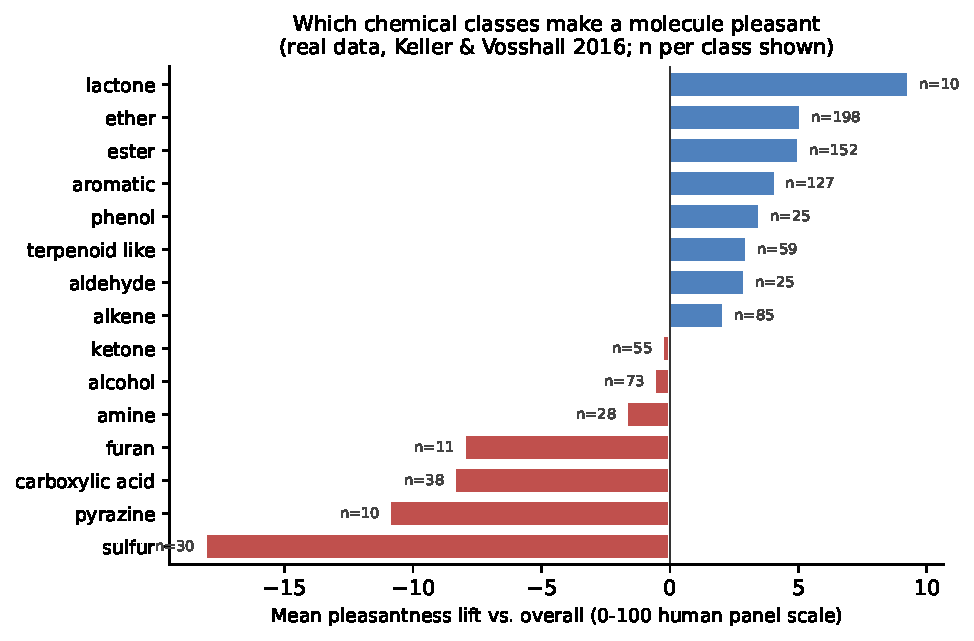
\includegraphics[width=0.72\linewidth]{class_pleasantness.pdf}
\caption{Chemical-class pleasantness lifts learned from real human-panel data (Keller \&
Vosshall 2016). Lactones, ethers, esters, aromatics, and phenols raise pleasantness; sulfur,
pyrazine, carboxylic-acid, and furan groups lower it. These data-driven lifts define the target
composition used to steer recipe generation, and recover well-known flavor chemistry.}
\label{fig:classlift}
\end{figure}

\begin{table}[h]\centering
\begin{tabular}{lll}
\toprule
Component & Metric & Value \\
\midrule
Structure $\to$ human pleasantness & 5-fold CV Spearman / $R^2$ & $0.50$ / $0.26$ \\
Learned mixture vs mean-pool & Spearman & $0.82$ vs $0.25$ \\
Molecule $\to$ receptor (Mainland) & vs chance & $1.57\times$ \\
Composition $\to$ blend pleasantness & Spearman & $0.42$ \\
Toxicity screen & molecules passing & $380/420$ \\
De-novo molecules & safe \& novel; top-12 in PubChem & $434$; $0/12$ \\
Metric best-part bound & Lean machine-checked & exit $0$ \\
\bottomrule
\end{tabular}
\caption{Summary of validated results. All reproducible from the released code.}
\end{table}

Class-level statistics recover known flavor chemistry: lactones ($+9.3$), ethers, esters,
aromatics, phenols raise pleasantness; sulfur ($-18.1$), pyrazines, acids, furans lower it. The
final composition-guided generator yields blends with $6$--$8$ of $10$ components being de-novo
molecules, chemical novelty $0.63$--$0.67$ from all reference flavors.

\section{Limitations}
Pleasantness is only moderately predictable from structure ($R^2 = 0.26$); the additive combo
score is a first-order estimate; the mixture model is validated on a synthetic (if principled)
oracle because public mixture-pleasantness data are scarce; de-novo predictions are
extrapolation and are reported with nearest-known similarity; receptor coverage is sparse;
and novelty is relative to public data. Most importantly, tastiness is empirical: no result
here establishes that a physical blend tastes good.

\section{Broader impacts and safety}
The safety screen is a structural hazard filter, not a regulatory clearance; de-novo molecules
have no safety data. Outputs are hypotheses for expert evaluation, and the repository includes a
handoff document requiring GRAS/FEMA confirmation and dose limits before any human exposure.

\section{Reproducibility}
All data are public (via Pyrfume); all models, controls, and the Lean proof are released with
per-result JSON artifacts and a step-by-step replication guide.

\section{Conclusion}
We present an honest, end-to-end, reproducible instrument for novel flavor design that links
molecular structure, receptor activation, perception, and toxicity, with a machine-checked
metric property clarifying the role of non-additive modeling. The natural next step is wet-lab
and human-panel validation of the top candidates.

\begin{thebibliography}{9}
\bibitem{keller2016} Keller, A. and Vosshall, L.B. (2016). Olfactory perception of chemically
diverse molecules. \emph{BMC Neuroscience}.
\bibitem{dream} Keller, A. et al. (2017). Predicting human olfactory perception from chemical
features of odor molecules. \emph{Science}.
\bibitem{pom} Lee, B.K. et al. (2023). A principal odor map unifies diverse tasks in olfactory
perception. \emph{Science} 381:999--1006.
\bibitem{qian} Qian, W.W. et al. (2023). Metabolic activity organizes olfactory
representations. \emph{eLife} 12:e82502.
\bibitem{mainland} Mainland, J.D. et al. (2015). Human olfactory receptor responses to odorants.
\emph{Scientific Data / Nature Neuroscience}.
\bibitem{leffingwell} Leffingwell odor dataset; and Pyrfume: Castro, J.B. et al. (2024). A
window to the world's olfactory data. \emph{Scientific Data}.
\bibitem{duchamp} Duchamp-Viret, P. et al. (2003). Single olfactory sensory neurons
simultaneously integrate the components of an odour mixture. \emph{Eur. J. Neuroscience}.
\bibitem{barnum} Barnum, G. and Hong, E.J. (2022). Olfactory coding. \emph{Current Biology}
32:R1296--R1301.
\bibitem{brics} Degen, J. et al. (2008). On the art of compiling and using drug-like chemical
fragment spaces (BRICS). \emph{ChemMedChem}.
\bibitem{lean} Moura, L. de and Ullrich, S. (2021). The Lean 4 theorem prover and programming
language. \emph{CADE}.
\end{thebibliography}

\end{document}
